\documentclass[11pt]{article}

\usepackage[margin=2.2cm]{geometry}
\usepackage{xcolor}
\usepackage{forest}
\usepackage{tikz}
\usetikzlibrary{arrows.meta,positioning,decorations.pathreplacing,calc}
\usepackage{amsmath,amssymb,mathtools}
\usepackage{booktabs}
\usepackage{array}
\usepackage{enumitem}
\usepackage{titlesec}
\usepackage{float}
\usepackage[colorlinks=true,linkcolor=teal!70!black,citecolor=teal,urlcolor=teal]{hyperref}
\usepackage{parskip}

\setlength{\parskip}{0.5\baselineskip}
\titlespacing*{\section}{0pt}{1.5em}{0.6em}
\titlespacing*{\subsection}{0pt}{1.2em}{0.4em}

% ---- colors reused across every figure, so the same idea always wears the same color ----
\definecolor{lossless}{HTML}{1f7a6c}   % teal family
\definecolor{lossy}{HTML}{c2622d}      % orange family
\definecolor{prefixcol}{HTML}{6a4c93}  % violet
\definecolor{nonprefixcol}{HTML}{1f6fb2}% blue
\definecolor{dictcol}{HTML}{8a5a2b}    % brown
\definecolor{bestcol}{HTML}{2e8b3d}    % green, "best in class" marker
\definecolor{warncol}{HTML}{b3261e}    % red, "error / impossible" marker
\definecolor{transformcol}{HTML}{2f7d8f}% steel teal, transform-based family
\definecolor{contextcol}{HTML}{a13d63} % magenta, context-modeling family
\definecolor{mmcol}{HTML}{4f6d2f}      % olive, lossless multimedia family

\newcommand{\figdrawnote}[1]{\par\noindent\textbf{\textcolor{gray!60!black}{[Draw on the board here:}} \textit{#1}\textbf{\textcolor{gray!60!black}{]}}\par}

% ---- a colored callout box for direct-to-camera, pause-and-think moments ----
\newcommand{\engage}[3]{%
\begin{center}
\begin{tikzpicture}
\node[draw=#1, thick, rounded corners, fill=#1!6, align=left,
      font=\sffamily\small, text width=0.92\linewidth, inner sep=9pt]
      {\textbf{\textcolor{#1}{#2}}\; #3};
\end{tikzpicture}
\end{center}
}

\title{\Large\bfseries Data Compression Overview\\[4pt]
\large\normalfont Video script with synchronized blackboard figures}
\author{}
\date{}

\begin{document}
\maketitle
\vspace{-2em}

\noindent This is the narration script for the video, with every figure placed exactly
where it should be drawn. Figures that build up over the course of the video
(the master tree, the Shannon-limit wall) appear more than once, each time
showing only what should be on the board \emph{at that point} -- draw onto the
same space rather than starting over.

\section*{Part 1 --- Lossless vs. lossy}

This video gives you a bird's eye view of data compression algorithms and
techniques. We won't go deep into any single algorithm here. But this high
level view is critical. It helps you understand the overall field of data
compression. And it shows you where everything we cover in this course
actually fits. Throughout the video you'll see a series of tree diagrams.
These show the hierarchy of compression algorithms and techniques. Here is
the first one.

As this diagram shows, every data compression algorithm falls into one of
two broad categories. These are lossless and lossy.

\begin{figure}[H]
\centering
\begin{forest}
for tree={
  draw, rounded corners, align=center, l sep+=12pt, s sep+=14pt,
  edge={-{Latex[length=2mm]}}, anchor=north, child anchor=north,
  font=\sffamily\small, inner sep=5pt
}
[Data compression, fill=gray!10, draw=gray!70
  [Lossless, fill=lossless!12, draw=lossless]
  [Lossy, fill=lossy!12, draw=lossy]
]
\end{forest}
\caption*{\textbf{Figure 1a.} The master tree, stage 1. Just the root and the
two top-level branches -- this same tree keeps growing for the rest of the
video.}
\end{figure}

Let's understand exactly what separates these two categories. For that,
let's look at a simple block diagram.

Imagine you have some original data. We'll call it $x$. This data goes into
a compressor, also called an encoder. What comes out the other side is a
smaller, compressed version of that data. We'll call it $c$. Later, when you
want your data back, you take that compressed data $c$ and feed it into a
decompressor, also called a decoder. What comes out is the recovered data.
We'll call it $\bar{x}$.

\begin{figure}[H]
\centering
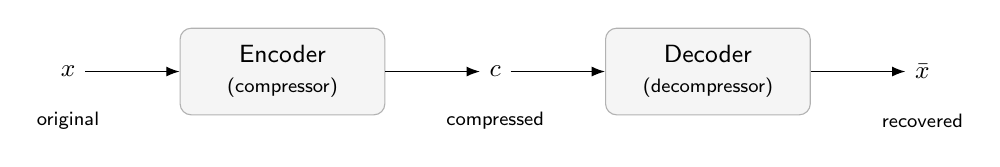
\begin{tikzpicture}[
  box/.style={draw, rounded corners, align=center, font=\sffamily\small, inner sep=6pt, minimum height=1.1cm, minimum width=2.6cm},
  lbl/.style={font=\sffamily\small},
  >=Latex
]
\node[lbl] (x) {$x$};
\node[box, right=12mm of x, fill=gray!8, draw=gray!60] (enc) {Encoder\\{\scriptsize (compressor)}};
\node[lbl, right=12mm of enc] (c) {$c$};
\node[box, right=12mm of c, fill=gray!8, draw=gray!60] (dec) {Decoder\\{\scriptsize (decompressor)}};
\node[lbl, right=12mm of dec] (xbar) {$\bar{x}$};

\draw[->] (x) -- (enc);
\draw[->] (enc) -- (c);
\draw[->] (c) -- (dec);
\draw[->] (dec) -- (xbar);

\node[font=\sffamily\scriptsize, below=2mm of x] {original};
\node[font=\sffamily\scriptsize, below=2mm of c] {compressed};
\node[font=\sffamily\scriptsize, below=2mm of xbar] {recovered};
\end{tikzpicture}
\caption*{\textbf{Figure 2.} The encoder/decoder pipeline. Every other figure
in this video about lossless vs.\ lossy is really just zooming in on what
happens to $\bar{x}$ at the very end of this diagram.}
\end{figure}

The entire difference between lossless and lossy compression comes down to
one question. How does $\bar{x}$ compare to the original $x$. In lossless
compression, $\bar{x}$ is always identical to $x$. No matter what the input
was, you are guaranteed to get back the exact original data, bit for bit. In
lossy compression, $\bar{x}$ is not identical to $x$. Some information was
discarded during the encoding process. That information is gone for good. So
what you get back is only an approximation of the original. It is not an
exact copy.

\begin{figure}[H]
\centering
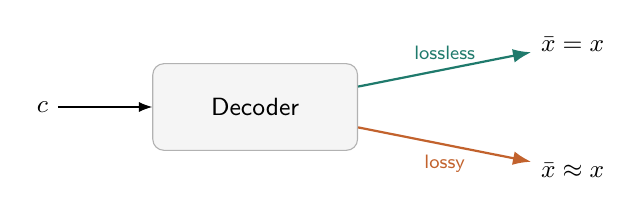
\begin{tikzpicture}[
  box/.style={draw, rounded corners, align=center, font=\sffamily\small, inner sep=6pt, minimum height=1.1cm, minimum width=2.6cm},
  lbl/.style={font=\sffamily\small},
  >=Latex
]
\node[box, fill=gray!8, draw=gray!60] (dec) {Decoder};
\node[lbl, left=12mm of dec] (c) {$c$};
\draw[->] (c) -- (dec);

\node[lbl, right=22mm of dec, yshift=8mm] (los) {$\bar{x} = x$};
\node[lbl, right=22mm of dec, yshift=-8mm] (lossy) {$\bar{x} \approx x$};

\draw[->, lossless, thick] (dec) -- (los) node[midway, above, font=\sffamily\scriptsize, lossless] {lossless};
\draw[->, lossy, thick] (dec) -- (lossy) node[midway, below, font=\sffamily\scriptsize, lossy] {lossy};
\end{tikzpicture}
\caption*{\textbf{Figure 3.} The fork that defines the whole field: exact
recovery (teal, lossless) or approximate recovery (orange, lossy). This
annotation sits directly on top of Figure 2's decoder output.}
\end{figure}

It makes sense to use lossy compression when the data is multimedia. That
means audio, video, or images. Losing some data in exchange for better
compression might not even be visible to the naked eye. It might not even be
audible to human ears. But in every other case, you need the data to come
back exactly as it was. Think of the textual records of government
employees. In those cases, you resort to lossless compression instead.

\section*{Part 2 --- The Shannon limit}

Before we divide lossless compression into its different categories, let's
first discuss one fundamental idea. It is one of the greatest theoretical
results in data compression. It is called the Shannon limit.

Claude Shannon showed that every source of data has a compression limit.
This is the maximum amount by which the data can be compressed without
losing any information. The limit depends on the amount of information, or
uncertainty, in the source. This quantity is called entropy.

\begin{figure}[H]
\centering
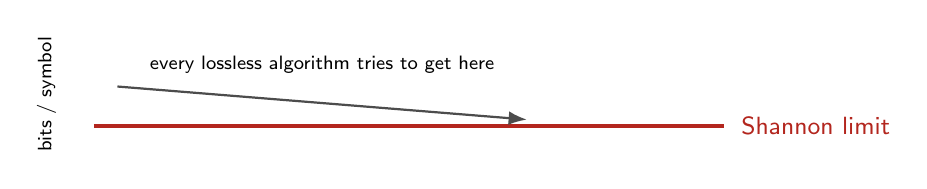
\begin{tikzpicture}[
  >=Latex, font=\sffamily\small
]
\draw[warncol, very thick] (0,0) -- (8,0);
\node[warncol, right] at (8.1,0) {Shannon limit};
\draw[->, gray!60!black, thick] (0.3,0.5) -- (5.5,0.08);
\node[font=\sffamily\scriptsize, above] at (2.9,0.55) {every lossless algorithm tries to get here};
\node[font=\sffamily\scriptsize, rotate=90] at (-0.6,0.4) {bits / symbol};
\end{tikzpicture}
\caption*{\textbf{Figure 4a.} The Shannon limit, stage 1: a wall that no
lossless algorithm can cross, with one generic arrow approaching it. No
specific algorithms yet -- those get added to this same wall much later, in
Figure 4b.}
\end{figure}

I have separate videos on entropy and the Shannon limit, so I won't discuss
them in detail here. The key idea is simple. No lossless compression
algorithm, no matter how clever, can achieve an average compressed size
below this limit.

So although the algorithms we are about to study are very different, they
all have the same goal. They try to compress data as close to the Shannon
limit as possible while remaining fast and memory efficient.

\section*{Part 3 --- The four families of lossless compression}

With that in mind, lossless compression can be divided into four categories.
Number one, entropy coding. Number two, dictionary or LZ family. Number
three, transform based compression. And number four, context modeling.

Let us first briefly describe each of these categories. Then we will zoom
into each one and build more tree diagrams.

\begin{figure}[H]
\centering
\begin{forest}
for tree={
  draw, rounded corners, align=center, l sep+=12pt, s sep+=10pt,
  edge={-{Latex[length=2mm]}}, anchor=north, child anchor=north,
  font=\sffamily\small, inner sep=5pt
}
[Data compression, fill=gray!10, draw=gray!70
  [Lossless, fill=lossless!12, draw=lossless
    [Entropy\\coding, fill=lossless!6, draw=lossless!70]
    [Dictionary\\/ LZ, fill=lossless!6, draw=lossless!70]
    [Transform\\based, fill=lossless!6, draw=lossless!70]
    [Context\\modeling, fill=lossless!6, draw=lossless!70]
  ]
  [Lossy, fill=lossy!12, draw=lossy]
]
\end{forest}
\caption*{\textbf{Figure 5.} The master tree, stage 2: Lossless gains its
four children. Lossy is still left empty on purpose -- it is not covered in
this video.}
\end{figure}

Let's start with entropy coding. Entropy coding is a family of techniques.
These techniques assign shorter codes to more probable symbols. They assign
longer codes to less probable ones. For example, in English text, the letter
$e$ appears much more often than the letter $x$. So an entropy coder would
assign a shorter code to $e$. It would assign a longer code to $x$.

\begin{figure}[H]
\centering
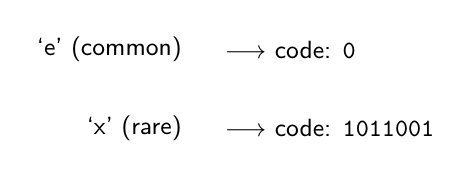
\begin{tikzpicture}[font=\sffamily\small]
\node[anchor=east] at (0,0.5) {`e' (common)};
\node[anchor=west] at (0.3,0.5) {$\longrightarrow$ code: \texttt{0}};
\node[anchor=east] at (0,-0.5) {`x' (rare)};
\node[anchor=west] at (0.3,-0.5) {$\longrightarrow$ code: \texttt{1011001}};
\end{tikzpicture}
\caption*{\textbf{Figure 6.} The intuition behind every entropy coder, before
any formal definitions: common symbols get short codes, rare symbols get
long ones.}
\end{figure}

This idea is actually quite intuitive. Symbols that occur more frequently
should take fewer bits to represent. Symbols that occur less frequently can
afford to use more bits. As a result, the average number of bits per symbol
goes down. This is how entropy coding approaches the Shannon limit we just
talked about.

\section*{Part 4 --- Entropy coding: prefix vs. non-prefix}

If we zoom into entropy coding, we find two further groups of algorithms.
These are prefix coding and non-prefix coding.

\begin{figure}[H]
\centering
\begin{forest}
for tree={
  draw, rounded corners, align=center, l sep+=12pt, s sep+=10pt,
  edge={-{Latex[length=2mm]}}, anchor=north, child anchor=north,
  font=\sffamily\small, inner sep=5pt
}
[Entropy coding, fill=lossless!10, draw=lossless!70
  [Prefix coding\\{\scriptsize whole-bit codewords}, fill=prefixcol!10, draw=prefixcol]
  [Non-prefix coding\\{\scriptsize fractional-bit codewords}, fill=nonprefixcol!10, draw=nonprefixcol]
]
\end{forest}
\caption*{\textbf{Figure 7.} The master tree, stage 3: Entropy Coding gains
its two children. Violet = prefix coding, blue = non-prefix coding -- these
two colors are reused for the rest of the entropy-coding section.}
\end{figure}

A prefix code is a type of code where no codeword is the prefix of any other
codeword. This means you can read a stream of bits from left to right. And
you can always tell exactly where one codeword ends. There is no ambiguity.

For example, consider this mapping. $A$ is encoded as \texttt{0}. $B$ is
encoded as \texttt{10}. $C$ is encoded as \texttt{110}. $D$ is encoded as
\texttt{111}. This is a prefix code. None of these codewords starts with
another complete codeword.

\begin{figure}[H]
\centering
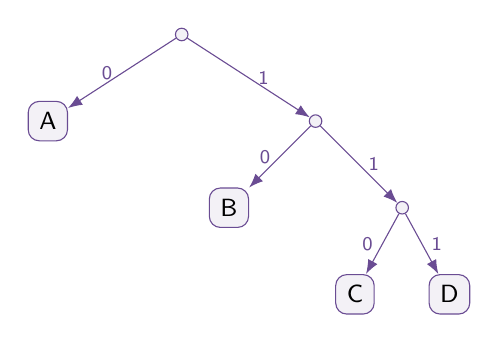
\begin{tikzpicture}[
  level distance=11mm,
  every node/.style={font=\sffamily\small},
  edge from parent/.style={draw, -{Latex[length=1.8mm]}, prefixcol},
  level 1/.style={sibling distance=34mm},
  level 2/.style={sibling distance=22mm},
  level 3/.style={sibling distance=12mm},
  leaf/.style={draw, rounded corners, fill=prefixcol!8, draw=prefixcol, inner sep=4pt},
  internal/.style={circle, draw=prefixcol, fill=prefixcol!8, inner sep=1.6pt}
]
\node[internal] (root) {}
  child { node[leaf] {A} edge from parent node[left, font=\sffamily\scriptsize] {0} }
  child { node[internal] (n1) {}
    child { node[leaf] {B} edge from parent node[left, font=\sffamily\scriptsize] {0} }
    child { node[internal] (n2) {}
      child { node[leaf] {C} edge from parent node[left, font=\sffamily\scriptsize] {0} }
      child { node[leaf] {D} edge from parent node[right, font=\sffamily\scriptsize] {1} }
      edge from parent node[right, font=\sffamily\scriptsize] {1}
    }
    edge from parent node[right, font=\sffamily\scriptsize] {1}
  };
\end{tikzpicture}
\caption*{\textbf{Figure 8.} A valid prefix code as a binary tree: $A=0$,
$B=10$, $C=110$, $D=111$. Every letter is a \emph{leaf} -- none of them sits
on the path to another letter, which is exactly what ``prefix-free'' means.}
\end{figure}

Now consider this mapping instead. $A$ is encoded as \texttt{0}. $B$ is
encoded as \texttt{01}. $C$ is encoded as \texttt{10}. $D$ is encoded as
\texttt{11}. This is not a prefix code. The codeword for $A$, which is
\texttt{0}, is a prefix of the codeword for $B$, which is \texttt{01}. This
creates ambiguity when decoding.

\begin{figure}[H]
\centering
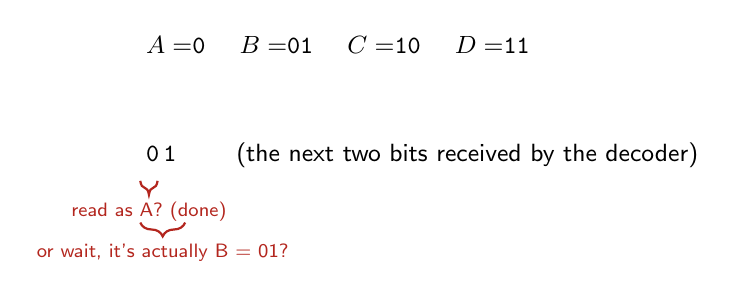
\begin{tikzpicture}[font=\sffamily\small]
\node[anchor=west] (mapping) at (0,1.4) {$A=$\texttt{0} \quad $B=$\texttt{01} \quad $C=$\texttt{10} \quad $D=$\texttt{11}};

\node[anchor=west] (bits) at (0,0) {\texttt{0}\,\texttt{1} \quad\quad (the next two bits received by the decoder)};

\draw[warncol, thick, decorate, decoration={brace, amplitude=5pt, mirror}] (0.05,-0.32) -- (0.27,-0.32) node[midway, below=4pt, warncol, font=\sffamily\scriptsize] {read as A? (done)};
\draw[warncol, thick, decorate, decoration={brace, amplitude=5pt, mirror}] (0.05,-0.85) -- (0.62,-0.85) node[midway, below=4pt, warncol, font=\sffamily\scriptsize] {or wait, it's actually B = 01?};
\end{tikzpicture}
\caption*{\textbf{Figure 9.} Why this mapping is ambiguous: after seeing the
single bit \texttt{0}, the decoder cannot tell whether to stop (it's $A$) or
keep reading (it might be the start of $B=01$). This is the one ``error''
figure in the section, marked in red.}
\end{figure}

Among prefix coding algorithms, we have Huffman coding, Shannon coding, and
Shannon Fano coding. Huffman coding is fast and simple to build. It is also
optimal among all prefix codes for a memoryless source. But Huffman coding is
not necessarily the best possible entropy coder in an absolute sense. Prefix
codes are constrained by the Kraft McMillan inequality. We will discuss that
in a separate video. One important consequence of this constraint is that
every codeword must have an integer number of bits. In our earlier example,
$A$ was assigned a code of length 1. $B$ was assigned a code of length 2. $C$
and $D$ were both assigned codes of length 3. These lengths are all integers.
We cannot assign $D$ a code of length 2.4 in Huffman coding.

Because of this restriction, Huffman coding cannot always match the exact
entropy of the source. So it cannot always reach the Shannon limit.
Arithmetic coding is different. It is a non-prefix entropy coding method. It
can assign each symbol a code of fractional length. So in our example, a
symbol like $D$ could actually be assigned a code of length 2.4.

\begin{figure}[H]
\centering
\begin{tabular}{@{}lcc@{}}
\toprule
\textbf{Symbol} & \textbf{Huffman (prefix)} & \textbf{Arithmetic (non-prefix)} \\
\midrule
$A$ & 1 bit & 1.1 bits \\
$B$ & 2 bits & 1.9 bits \\
$C$ & 3 bits & 2.7 bits \\
$D$ & 3 bits & \textcolor{warncol}{\textbf{2.4 bits}} \\
\bottomrule
\end{tabular}
\caption*{\textbf{Figure 10.} Why Huffman can't always reach the entropy
limit: every Huffman codeword length is a whole number (violet column), while
a non-prefix coder like Arithmetic coding can use fractional lengths (blue
column) -- a length of 2.4 bits, marked in red, is simply impossible for $D$
under Huffman coding.}
\end{figure}

Because of this, arithmetic coding can often get very close to the Shannon
limit. In many cases it gets closer than Huffman coding does. This means it
can offer a noticeably better compression ratio. But arithmetic coding is
also noticeably slower. It relies on fractional arithmetic, including
division. To solve this problem, researchers developed range coding. Range
coding uses only integer arithmetic. It avoids division entirely. Range
coding gives you exactly the same compression ratio as arithmetic coding.
But it runs faster.

More recently, many streaming applications have started using entropy
coding. One example is Zstandard, which is used by companies like Netflix and
YouTube. For these applications, even range coding is not fast enough. Users
could experience an annoying delay during streaming. To solve this,
researchers developed a family of algorithms called ANS. These are faster
than both arithmetic coding and range coding. But that extra speed comes at a
small cost. ANS gives you a slightly lower compression ratio in exchange,
very close to arithmetic and range coding but not quite as good. Within this
family, rANS, which stands for range ANS, is best suited for parallel
computing. Most streaming compression tools instead use tANS, which stands
for table ANS. tANS is the fastest of them all, since both encoding and
decoding reduce to simple table lookups.

\begin{figure}[H]
\centering
\begin{forest}
for tree={
  draw, rounded corners, align=center, l sep+=12pt, s sep+=8pt,
  edge={-{Latex[length=2mm]}}, anchor=north, child anchor=north,
  font=\sffamily\small, inner sep=5pt
}
[Entropy coding, fill=lossless!10, draw=lossless!70
  [Prefix coding, fill=prefixcol!10, draw=prefixcol
    [Huffman\\{\scriptsize fast, lowest ratio}, fill=prefixcol!6, draw=prefixcol]
  ]
  [Non-prefix coding, fill=nonprefixcol!10, draw=nonprefixcol
    [Arithmetic\\{\scriptsize best ratio, slowest}, fill=nonprefixcol!6, draw=nonprefixcol]
    [Range coding\\{\scriptsize best ratio, faster}, fill=nonprefixcol!6, draw=nonprefixcol]
    [rANS\\{\scriptsize near-best, fast, parallel}, fill=nonprefixcol!6, draw=nonprefixcol]
    [tANS\\{\scriptsize near-best, fastest}, fill=bestcol!12, draw=bestcol]
  ]
]
\end{forest}
\caption*{\textbf{Figure 7b.} The entropy-coding branch, fully grown. Green
marks tANS as the fastest of the five -- pure table lookups, no arithmetic at
all.}
\end{figure}

So here is how these five entropy coders actually compare. Huffman is the
quickest and simplest to build, but it gives up the most compression ratio,
since it's stuck with whole numbers of bits. Arithmetic coding and range
coding sit at the other end. They give you the best possible compression
ratio, right up against the Shannon limit. Between the two, range coding is
faster than arithmetic coding, since it avoids division. rANS and tANS sit in
between on ratio, very close to arithmetic and range coding but not quite as
good, and they are the fastest of the group when it comes to actually running
the encoder and decoder, with tANS being the fastest of all since it relies
purely on table lookups.

\begin{figure}[H]
\centering
\begin{tikzpicture}[font=\sffamily\small, >=Latex]
\draw[->, thick] (0,0) -- (0,5.2) node[above, font=\sffamily\small] {compression ratio (best $\uparrow$)};
\draw[->, thick] (0,0) -- (9.2,0) node[right, font=\sffamily\small] {speed (fastest $\rightarrow$)};

% Huffman: lowest ratio
\filldraw[prefixcol] (1.4,1.0) circle (2.2pt);
\node[anchor=west, prefixcol] at (1.6,1.0) {Huffman};

% Arithmetic and Range: tied, best ratio
\filldraw[nonprefixcol] (3.0,4.6) circle (2.2pt);
\node[anchor=south, nonprefixcol] at (3.0,4.75) {Arithmetic};
\filldraw[nonprefixcol] (4.6,4.6) circle (2.2pt);
\node[anchor=south, nonprefixcol] at (4.6,4.75) {Range};

% rANS, tANS: slightly below Arithmetic/Range on ratio, faster
\filldraw[nonprefixcol] (6.2,3.5) circle (2.2pt);
\node[anchor=west, nonprefixcol] at (6.4,3.5) {rANS};
\filldraw[bestcol] (8.0,3.5) circle (2.2pt);
\node[anchor=west, bestcol] at (8.2,3.5) {tANS};
\end{tikzpicture}
\caption*{\textbf{Figure 11.} Speed vs.\ compression ratio for all five
entropy coders. Two details that are easy to get backwards: Range sits to the
\emph{right} of (faster than) Arithmetic at the \emph{same} height (same
ratio), and Huffman's defining trait here is the \emph{lowest ratio}, not the
fastest runtime -- tANS (green) is the fastest-running coder of the five.}
\end{figure}

\begin{figure}[H]
\centering
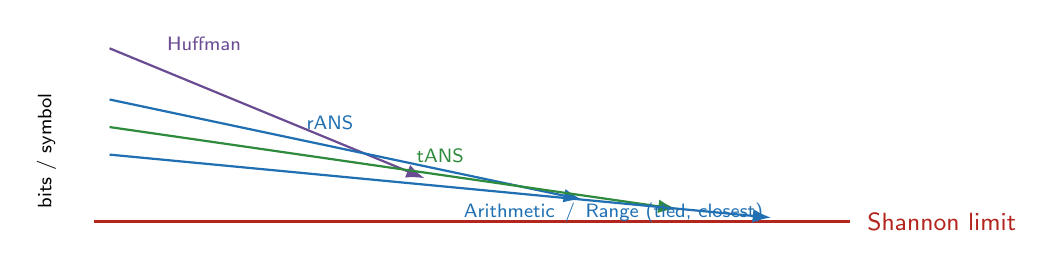
\begin{tikzpicture}[
  >=Latex, font=\sffamily\small
]
\draw[warncol, very thick] (0,0) -- (9.6,0);
\node[warncol, right] at (9.7,0) {Shannon limit};
\node[font=\sffamily\scriptsize, rotate=90] at (-0.6,0.9) {bits / symbol};

\draw[->, prefixcol, thick] (0.2,2.2) -- (4.2,0.55);
\node[prefixcol, font=\sffamily\scriptsize, above] at (1.4,2.05) {Huffman};

\draw[->, nonprefixcol, thick] (0.2,1.55) -- (6.2,0.28);
\node[nonprefixcol, font=\sffamily\scriptsize, above] at (3.0,1.05) {rANS};

\draw[->, bestcol, thick] (0.2,1.2) -- (7.4,0.16);
\node[bestcol, font=\sffamily\scriptsize, above] at (4.4,0.62) {tANS};

\draw[->, nonprefixcol, thick] (0.2,0.85) -- (8.6,0.05);
\node[nonprefixcol, font=\sffamily\scriptsize, below=1pt] at (6.6,0.40) {Arithmetic \,/\, Range (tied, closest)};
\end{tikzpicture}
\caption*{\textbf{Figure 4b.} The Shannon limit wall, fully labeled. Arithmetic
and Range coding are tied for closest to the limit -- that is the entire
reason they exist. rANS and tANS trade a small, deliberate gap from the limit
for a large gain in speed. Huffman is furthest from the wall, since it is
locked into whole-bit codewords. Colors match Figure 7b.}
\end{figure}

\section*{Part 5 --- Dictionary compression: the LZ family}

Now next we move to dictionary based compression algorithms. They mostly
belong to the LZ family. At a high level, we can divide them into LZ77 and
LZ78.

\begin{figure}[H]
\centering
\begin{forest}
for tree={
  draw, rounded corners, align=center, l sep+=12pt, s sep+=10pt,
  edge={-{Latex[length=2mm]}}, anchor=north, child anchor=north,
  font=\sffamily\small, inner sep=5pt
}
[Data compression, fill=gray!10, draw=gray!70
  [Lossless, fill=lossless!12, draw=lossless
    [Entropy\\coding, fill=lossless!6, draw=lossless!70]
    [Dictionary\\/ LZ, fill=dictcol!10, draw=dictcol
      [LZ77\\{\scriptsize sliding window}, fill=dictcol!6, draw=dictcol]
      [LZ78\\{\scriptsize growing dictionary}, fill=dictcol!6, draw=dictcol]
    ]
    [Transform\\based, fill=lossless!6, draw=lossless!70]
    [Context\\modeling, fill=lossless!6, draw=lossless!70]
  ]
  [Lossy, fill=lossy!12, draw=lossy]
]
\end{forest}
\caption*{\textbf{Figure 12.} The master tree, stage 4: Dictionary / LZ gains
its two children, LZ77 and LZ78, drawn in a new color (brown) so it's
visually distinct from the entropy-coding branch.}
\end{figure}

The key difference is this. LZ77 uses a sliding window. This makes it memory
constrained. LZ78 instead uses a growing dictionary.

\begin{figure}[H]
\centering
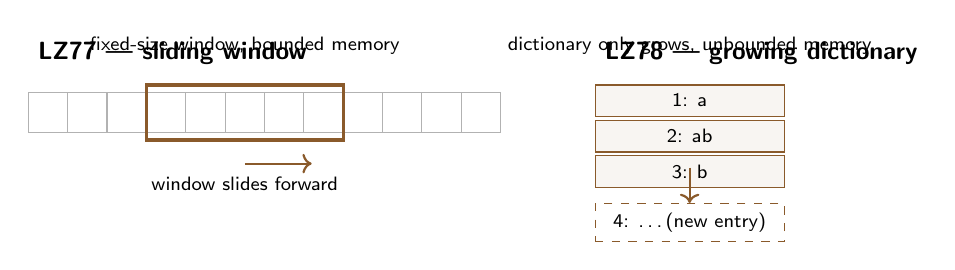
\begin{tikzpicture}[font=\sffamily\small]
% LZ77: sliding window over a fixed-length tape
\node[anchor=west] at (0,3.0) {\textbf{LZ77 --- sliding window}};
\foreach \i in {0,...,11}{
  \draw[gray!60] (\i*0.5,2.0) rectangle (\i*0.5+0.5,2.5);
}
\draw[dictcol, very thick] (1.5,1.9) rectangle (4.0,2.6);
\draw[->, dictcol, thick] (2.75,1.6) -- (3.6,1.6);
\node[font=\sffamily\scriptsize, below] at (2.75,1.55) {window slides forward};
\node[font=\sffamily\scriptsize] at (2.75,3.5) [yshift=-0.4cm] {fixed-size window, bounded memory};

% LZ78: growing dictionary table
\node[anchor=west] at (7.2,3.0) {\textbf{LZ78 --- growing dictionary}};
\foreach \i/\txt in {0/1: a, 1/2: ab, 2/3: b}{
  \node[draw=dictcol, fill=dictcol!6, font=\sffamily\scriptsize, minimum width=2.4cm] at (8.4,2.4-\i*0.45) {\txt};
}
\draw[->, dictcol, thick] (8.4,1.55) -- (8.4,1.1);
\node[draw=dictcol, dashed, font=\sffamily\scriptsize, minimum width=2.4cm] at (8.4,0.85) {4: \ldots (new entry)};
\node[font=\sffamily\scriptsize] at (8.4,3.5) [yshift=-0.4cm] {dictionary only grows, unbounded memory};
\end{tikzpicture}
\caption*{\textbf{Figure 13.} The core contrast between the two LZ branches.
LZ77's window (left) stays the same size and slides over the data it has
already seen. LZ78's dictionary (right) starts empty and gains a new entry
every time a new substring is seen.}
\end{figure}

Most of the algorithms we cover in this course are extensions of LZ77. For
example, DEFLATE is LZ77 combined with Huffman coding. And Zstandard is LZ77
combined with tANS.

\begin{figure}[H]
\centering
\begin{forest}
for tree={
  draw, rounded corners, align=center, l sep+=12pt, s sep+=10pt,
  edge={-{Latex[length=2mm]}}, anchor=north, child anchor=north,
  font=\sffamily\small, inner sep=5pt
}
[LZ77, fill=dictcol!10, draw=dictcol
  [DEFLATE\\{\scriptsize LZ77 + \textcolor{prefixcol}{Huffman}}, fill=dictcol!6, draw=dictcol]
  [Zstandard\\{\scriptsize LZ77 + \textcolor{bestcol}{tANS}}, fill=dictcol!6, draw=dictcol]
]
\end{forest}
\caption*{\textbf{Figure 14.} LZ77 in practice: two real formats, each adding
an entropy coder from Part 4 at the very end. The ``+Huffman'' and ``+tANS''
labels are colored to match Figures 7b and 11 -- dictionary methods don't
replace entropy coding, they hand off to it.}
\end{figure}

\section*{Part 6 --- Transform-based compression: the Burrows--Wheeler Transform}

We've now covered two of our four lossless families: entropy coding and
dictionary compression. Let's move to the third family. Transform based
compression.

Here's the core idea. Instead of compressing the data directly, first
transform it into a completely different arrangement of the exact same
symbols. An arrangement that happens to be far easier to compress. Then run
a simple compressor on top of that.

The most famous example of this approach is the Burrows-Wheeler Transform,
or BWT. It is the engine inside the popular bzip2 compressor.

\engage{transformcol}{Pause and guess:}{the Burrows-Wheeler Transform, by
itself, does not save a single bit. Not one. So why would anyone bother
using it? Take a guess, then keep watching.}

Here's how it works. Take your string, and add a unique end marker to it,
say a dollar sign. Now generate every rotation of that string. Sort all of
those rotations alphabetically. The BWT output is simply the last column of
that sorted list.

\begin{figure}[H]
\centering
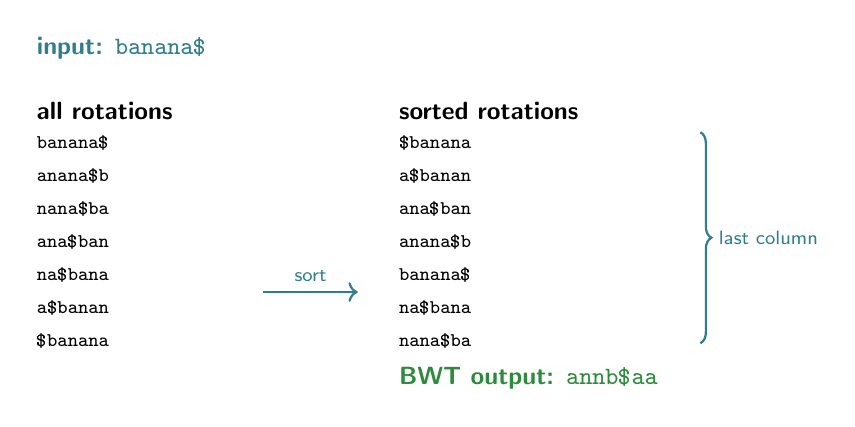
\begin{tikzpicture}[font=\sffamily\small]
\node[anchor=west, transformcol, font=\sffamily\small\bfseries] at (0,5.2) {input: \texttt{banana\$}};

\node[anchor=west] at (0,4.4) {\textbf{all rotations}};
\foreach \i/\txt in {0/banana\$,1/anana\$b,2/nana\$ba,3/ana\$ban,4/na\$bana,5/a\$banan,6/\$banana}{
  \node[font=\sffamily\scriptsize, anchor=west] at (0,4.0-\i*0.42) {\texttt{\txt}};
}

\draw[->, transformcol, thick] (3.0,2.1) -- (4.2,2.1) node[midway, above, font=\sffamily\scriptsize, transformcol] {sort};

\node[anchor=west] at (4.6,4.4) {\textbf{sorted rotations}};
\foreach \i/\txt in {0/\$banana,1/a\$banan,2/ana\$ban,3/anana\$b,4/banana\$,5/na\$bana,6/nana\$ba}{
  \node[font=\sffamily\scriptsize, anchor=west] at (4.6,4.0-\i*0.42) {\texttt{\txt}};
}

\draw[transformcol, thick, decorate, decoration={brace, amplitude=4pt}] (8.55,4.13) -- (8.55,1.45) node[midway, right=3pt, font=\sffamily\scriptsize, transformcol] {last column};

\node[anchor=west, bestcol, font=\sffamily\small\bfseries] at (4.6,1.0) {BWT output: \texttt{annb\$aa}};
\end{tikzpicture}
\caption*{\textbf{Figure 15.} The Burrows-Wheeler Transform of \texttt{banana\$},
worked by hand. Every rotation of the input (left) is sorted alphabetically
(right), and the last letter of each sorted row, read top to bottom, is the
BWT output. Notice the output has far more repeated, neighboring letters
than the original string did.}
\end{figure}

So why bother? Look closely at the output: \texttt{annb\$aa}. Compare that to
the original: \texttt{banana\$}. The letters haven't changed, and there are
exactly as many of them. But in the BWT output, identical letters are far
more likely to sit right next to each other. That's because sorting groups
together every rotation that shares the same upcoming context. The BWT
itself doesn't compress anything. What it does is rearrange the data so that
a much simpler compressor, typically a move-to-front transform, followed by
run-length encoding, followed by entropy coding, can squeeze it far harder
than it could squeeze the original. That handoff to a simple downstream
compressor is exactly how bzip2 is built.

\begin{figure}[H]
\centering
\begin{forest}
for tree={
  draw, rounded corners, align=center, l sep+=12pt, s sep+=10pt,
  edge={-{Latex[length=2mm]}}, anchor=north, child anchor=north,
  font=\sffamily\small, inner sep=5pt
}
[Transform\\based, fill=transformcol!10, draw=transformcol
  [BWT\\{\scriptsize\parbox{4.4cm}{\centering reorders symbols by context so simple coders can exploit the new runs; powers bzip2}}, fill=transformcol!6, draw=transformcol]
]
\end{forest}
\caption*{\textbf{Figure 16.} The transform-based branch. BWT doesn't compete
with entropy coding or LZ -- it's a pre-processing step that makes whatever
comes after it work better.}
\end{figure}

\section*{Part 7 --- Context modeling: PPM and context mixing}

That brings us to the fourth and final lossless family: context modeling.

Entropy coding, which we covered in Part 4, assigns a symbol's code length
based on how common that symbol is, overall, across the entire source.
Context modeling asks a sharper question. Forget the overall frequency. How
likely is this symbol to appear \emph{right here}, given the handful of
symbols that just came before it?

The flagship algorithm in this family is called PPM, which stands for
Prediction by Partial Matching.

\engage{contextcol}{Quick check:}{if entropy coding already gives common
symbols short codes, what extra trick is context modeling adding on top?
(Answer is in the next paragraph -- try to guess it first.)}

Here is PPM, in plain terms. To predict the next symbol, PPM looks at the
last few symbols it has already seen, that short, recent window is the
\emph{context}, the ``partial match.'' It then checks how often each
possible symbol has followed that exact context before, and turns those
counts into a probability distribution. That distribution gets handed to an
entropy coder, almost always arithmetic coding, which does the actual work
of writing out the bits. And if that exact context has never come up
before, PPM doesn't give up: it escapes down to a shorter context, one
symbol shorter at a time, until it finds one with real statistics behind it.

\begin{figure}[H]
\centering
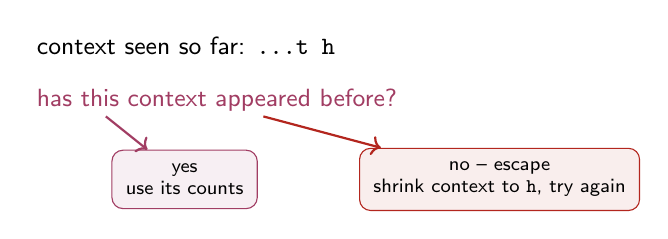
\begin{tikzpicture}[font=\sffamily\small]
\node[anchor=west] at (0,2.6) {context seen so far: \texttt{\ldots t h}};
\node[anchor=west, contextcol] at (0,1.9) {has this context appeared before?};

\node[draw=contextcol, rounded corners, fill=contextcol!8, align=center, font=\sffamily\scriptsize, inner sep=5pt] (yes) at (2.0,0.9) {yes\\use its counts};
\node[draw=warncol, rounded corners, fill=warncol!8, align=center, font=\sffamily\scriptsize, inner sep=5pt] (no) at (6.0,0.9) {no -- escape\\shrink context to \texttt{h}, try again};

\draw[->, contextcol, thick] (1.0,1.7) -- (yes);
\draw[->, warncol, thick] (3.0,1.7) -- (no);
\end{tikzpicture}
\caption*{\textbf{Figure 17.} PPM's escape mechanism. If the current context
has statistics, PPM uses them directly (left, teal-magenta). If not, it
shrinks the context by one symbol and tries again (right, red), repeating
until it lands on a context it has actually seen.}
\end{figure}

PPM has a more powerful, and much slower, cousin called context mixing, or
CM. Instead of picking one context length and falling back when it fails,
context mixing blends predictions from many different models at once,
different context lengths, even entirely different kinds of models, using a
weighted combination instead of an either-or choice. This family holds the
records for the best compression ratios ever measured, and it's the
approach behind compressors like PAQ and its descendants. The cost is speed:
context mixing can run hundreds of times slower than something like Huffman
coding.

\begin{figure}[H]
\centering
\begin{forest}
for tree={
  draw, rounded corners, align=center, l sep+=12pt, s sep+=10pt,
  edge={-{Latex[length=2mm]}}, anchor=north, child anchor=north,
  font=\sffamily\small, inner sep=5pt
}
[Context\\modeling, fill=contextcol!10, draw=contextcol
  [PPM\\{\scriptsize\parbox{4.4cm}{\centering predicts each symbol from its recent context, escaping to shorter contexts when needed}}, fill=contextcol!6, draw=contextcol]
  [Context\\mixing (CM)\\{\scriptsize\parbox{4.4cm}{\centering blends many context models at once; best ratio of all, but very slow}}, fill=bestcol!12, draw=bestcol]
]
\end{forest}
\caption*{\textbf{Figure 18.} The context-modeling branch. Context mixing
(green) sits at the extreme ``best possible ratio'' end of every trade-off
curve we've drawn so far, paid for entirely in speed.}
\end{figure}

\section*{Part 8 --- A fifth lossless branch: multimedia}

We've now met all four algorithmic families that make up lossless
compression: entropy coding, dictionary or LZ, transform based, and context
modeling. But there's one more branch worth adding under lossless, and it's
a slightly surprising one: multimedia.

Earlier in this video I said multimedia, video, images, and audio, is the
classic use case for \emph{lossy} compression. That's true most of the time.
But sometimes you cannot afford to lose anything: medical scans, film
archives, or a studio's master audio recording. For those cases, engineers
built dedicated lossless formats for video, images, and audio. And under the
hood, every one of them is just a clever combination of the four families we
already covered.

\engage{mmcol}{Pause and guess:}{FLAC is a lossless audio format. Based on
everything we've covered so far, which lossless family or families do you
think it leans on? Keep reading to check your guess.}

\begin{figure}[H]
\centering
\begin{forest}
for tree={
  draw, rounded corners, align=center, l sep+=10pt, s sep+=7pt,
  edge={-{Latex[length=2mm]}}, anchor=north, child anchor=north,
  font=\sffamily\small, inner sep=4pt
}
[Data compression, fill=gray!10, draw=gray!70
  [Lossless, fill=lossless!12, draw=lossless
    [Entropy\\coding, fill=lossless!6, draw=lossless!70]
    [Dictionary\\/ LZ, fill=dictcol!10, draw=dictcol]
    [Transform\\based, fill=transformcol!10, draw=transformcol]
    [Context\\modeling, fill=contextcol!10, draw=contextcol]
    [Multimedia, fill=mmcol!10, draw=mmcol
      [Video\\{\scriptsize FFV1}, fill=mmcol!6, draw=mmcol]
      [Image\\{\scriptsize PNG}, fill=mmcol!6, draw=mmcol]
      [Audio\\{\scriptsize FLAC}, fill=mmcol!6, draw=mmcol]
    ]
  ]
  [Lossy, fill=lossy!12, draw=lossy]
]
\end{forest}
\caption*{\textbf{Figure 19.} The master tree, stage 5: Lossless gains a
fifth child, Multimedia (olive), which in turn splits into the three media
types we keep coming back to -- video, image, and audio. Lossy is still
collapsed on purpose; we expand it in Part 9.}
\end{figure}

Let's take each one in turn.

\textbf{Lossless video -- FFV1.} FFV1 predicts each pixel from its
already-decoded neighbors, then entropy-codes the small leftover error with
range coding. It's the format film archives and broadcasters reach for when
a frame absolutely cannot change, not even by one pixel.

\textbf{Lossless images -- PNG.} PNG runs a per-row prediction filter to
exploit how similar neighboring pixels usually are, then compresses the
resulting residual with DEFLATE, the same LZ77-plus-Huffman pipeline from
Part 5.

\textbf{Lossless audio -- FLAC.} FLAC predicts each audio sample from the
samples just before it, then entropy-codes the small prediction error with
fast, simple Rice coding, a close cousin of the prefix codes from Part 4.

So if you guessed ``a transform-style prediction step followed by entropy
coding'' for FLAC, you were right. That same pattern, predict, then
entropy-code the error, shows up in FFV1 and PNG too. Multimedia formats
aren't a fifth way of compressing data. They're the first four families,
specialized for pixels and samples.

\section*{Part 9 --- Filling in lossy: video, images, and audio}

Now let's finally fill in the other half of our master tree: lossy
compression. Unlike lossless, lossy compression doesn't reduce neatly into
four shared families. Instead, it splits naturally by media type, because
what counts as ``unnoticeable'' is different for your eyes than it is for
your ears.

\textbf{Lossy images -- JPEG.} JPEG splits the image into small blocks,
transforms each block into frequency components with the discrete cosine
transform, and then throws away the high-frequency detail the human eye is
least likely to notice.

\textbf{Lossy audio -- MP3 / Opus.} These formats lean on a psychoacoustic
model, a model of what the human ear can and can't actually perceive, to
discard sound components you wouldn't hear anyway, then entropy-code
whatever's left.

\textbf{Lossy video -- H.264 / HEVC / AV1.} Video reuses the image trick at
its core: each frame still gets the block-transform-and-discard treatment.
But video adds one more move. It predicts each frame from neighboring
frames using motion estimation, so it only has to encode what actually
\emph{changed} between frames, not the whole picture over and over.

\engage{lossy}{Connect the dots:}{lossy video is really lossy image
compression, applied frame by frame, plus one new idea. Can you name that
new idea before reading the paragraph above again? (Hint: it's about what
changes \emph{between} frames, not within one.)}

\begin{figure}[H]
\centering
\begin{forest}
for tree={
  draw, rounded corners, align=center, l sep+=10pt, s sep+=10pt,
  edge={-{Latex[length=2mm]}}, anchor=north, child anchor=north,
  font=\sffamily\small, inner sep=5pt
}
[Lossy, fill=lossy!12, draw=lossy
  [Video\\{\scriptsize\parbox{4.0cm}{\centering H.264 / HEVC / AV1: motion-predicts frames, then transforms \\\& discards per frame}}, fill=lossy!6, draw=lossy]
  [Image\\{\scriptsize\parbox{4.0cm}{\centering JPEG / WebP: block DCT, discards high-frequency detail the eye misses}}, fill=lossy!6, draw=lossy]
  [Audio\\{\scriptsize\parbox{4.0cm}{\centering MP3 / AAC / Opus: discards sound a psychoacoustic model says you can't hear}}, fill=lossy!6, draw=lossy]
]
\end{forest}
\caption*{\textbf{Figure 20.} The lossy branch, fully grown. Video (left)
builds directly on the same per-frame transform trick used for still images
(middle), then adds motion prediction across frames. Audio (right) follows
the same overall pattern -- discard what perception can't catch -- using a
hearing model instead of a vision model.}
\end{figure}

\section*{Part 10 --- The complete tree}

We've now filled in every branch we set out to cover. Let's step back and
look at the whole thing, lossless and lossy, side by side, one last time.

\begin{figure}[H]
\centering
\resizebox{\textwidth}{!}{%
\begin{forest}
for tree={
  draw, rounded corners, align=center, l sep+=8pt, s sep+=4pt,
  edge={-{Latex[length=1.6mm]}}, anchor=north, child anchor=north,
  font=\sffamily\scriptsize, inner sep=3pt
}
[Lossless, fill=lossless!12, draw=lossless
  [Entropy\\coding, fill=lossless!6, draw=lossless!70
    [Prefix\\(Huffman), fill=prefixcol!8, draw=prefixcol]
    [Non-prefix\\(Arith./Range/rANS/tANS), fill=nonprefixcol!8, draw=nonprefixcol]
  ]
  [Dictionary\\/ LZ, fill=dictcol!10, draw=dictcol
    [{LZ77\\(DEFLATE, Zstandard)}, fill=dictcol!6, draw=dictcol]
    [LZ78, fill=dictcol!6, draw=dictcol]
  ]
  [Transform\\based, fill=transformcol!10, draw=transformcol
    [BWT\\(bzip2), fill=transformcol!6, draw=transformcol]
  ]
  [Context\\modeling, fill=contextcol!10, draw=contextcol
    [PPM, fill=contextcol!6, draw=contextcol]
    [CM, fill=bestcol!12, draw=bestcol]
  ]
  [Multimedia, fill=mmcol!10, draw=mmcol
    [Video (FFV1), fill=mmcol!6, draw=mmcol]
    [Image (PNG), fill=mmcol!6, draw=mmcol]
    [Audio (FLAC), fill=mmcol!6, draw=mmcol]
  ]
]
\end{forest}%
}
\caption*{\textbf{Figure 21a.} The complete tree, lossless half. Every
colored leaf here is something we built up piece by piece over Parts 3
through 8.}
\end{figure}

\begin{figure}[H]
\centering
\begin{forest}
for tree={
  draw, rounded corners, align=center, l sep+=12pt, s sep+=12pt,
  edge={-{Latex[length=1.8mm]}}, anchor=north, child anchor=north,
  font=\sffamily\small, inner sep=5pt
}
[Lossy, fill=lossy!12, draw=lossy
  [Video\\(H.264/HEVC/AV1), fill=lossy!6, draw=lossy]
  [Image\\(JPEG/WebP), fill=lossy!6, draw=lossy]
  [Audio\\(MP3/AAC/Opus), fill=lossy!6, draw=lossy]
]
\end{forest}
\caption*{\textbf{Figure 21b.} The complete tree, lossy half, from Part 9.
Lossy splits by medium instead of by algorithmic family, since what's
``unnoticeable'' depends on whether you're looking or listening.}
\end{figure}

And that's the full map. Two root branches, lossless and lossy, five
lossless families, and three media types under lossy. Every algorithm we
study for the rest of this course slots into one leaf of this tree. Whenever
you feel lost in a later video, come back to this picture and ask yourself:
which leaf am I in right now?

\end{document}
